\documentclass[
  digital, %% This option enables the default options for the
           %% digital version of a document. Replace with `printed`
           %% to enable the default options for the printed version
           %% of a document.
  notable,   %% Causes the coloring of tables. Replace with `notable`
           %% to restore plain tables.
  nolof,     %% Prints the List of Figures. Replace with `nolof` to
           %% hide the List of Figures.
  nolot,     %% Prints the List of Tables. Replace with `nolot` to
           %% hide the List of Tables.
  %% More options are listed in the user guide at
  %% <http://mirrors.ctan.org/macros/latex/contrib/fithesis/guide/mu/fi.pdf>.
]{fithesis3}
%% The following section sets up the locales used in the thesis.
\usepackage[resetfonts]{cmap} %% We need to load the T2A font encoding
\usepackage[T1,T2A]{fontenc}  %% to use the Cyrillic fonts with Russian texts.
\usepackage[
  main=english, %% By using `czech` or `slovak` as the main locale
                %% instead of `english`, you can typeset the thesis
                %% in either Czech or Slovak, respectively.
  german, russian, czech, slovak %% The additional keys allow
]{babel}        %% foreign texts to be typeset as follows:
\usepackage{acro}
%%
%%   \begin{otherlanguage}{german}  ... \end{otherlanguage}
%%   \begin{otherlanguage}{russian} ... \end{otherlanguage}
%%   \begin{otherlanguage}{czech}   ... \end{otherlanguage}
%%   \begin{otherlanguage}{slovak}  ... \end{otherlanguage}
%%
%% For non-Latin scripts, it may be necessary to load additional
%% fonts:
\usepackage{paratype}
\usepackage{overpic}
\def\textrussian#1{{\usefont{T2A}{PTSerif-TLF}{m}{rm}#1}}
%%
%% The following section sets up the metadata of the thesis.
\thesissetup{
    date          = \the\year/\the\month/\the\day,
    university    = mu,
    faculty       = fi,
    type          = mgr,
    author        = Samuel Pastva,
    gender        = m,
    advisor       = {prof. RNDr. Luboš Brim, CSc.},
    title         = {Parallel parameter synthesis from hybrid logic HUCTL formulas},
    TeXtitle      = {Parallel parameter synthesis from hybrid logic $HUCTL_{P}$ formulas},
    keywords      = {parameter synthesis, model checking, temporal logic, HUCTL, dynamical system, ordinary differential equation, parallel algorithm},
    TeXkeywords   = {parameter synthesis, model checking, temporal logic, $HUCTL_{P}$, dynamical system, ordinary differential equation, parallel algorithm},
    bib           = main.bib,
}

\usepackage{algorithmicx}

\usepackage{makeidx}      %% The `makeidx` package contains
\makeindex                %% helper commands for index typesetting.
%% These additional packages are used within the document:
\usepackage{paralist} %% Compact list environments
\usepackage{amsmath}  %% Mathematics
\usepackage{amsthm}
\usepackage{amsfonts}
\usepackage{url}      %% Hyperlinks

\newtheorem{definition}{Definition}
\newtheorem{lemma}{Lemma}
\newtheorem{theorem}{Theorem}

% Custom macros and definitions

\newcommand{\INIT}{\STATE \textbf{init} {}}
\newcommand{\df}{\scalebox{.9}{$\stackrel{{\tiny \mathrm{df}}}{=}$}}
\newcommand{\TBA}{{\bf TBA}}

\newcommand{\ptort}[1]{\mbox{$\stackrel{#1}{\rightarrow}\hspace{-.65ex}%
		\raisebox{.15em}{\scriptsize *}\hspace{.65ex}$}}
\newcommand{\ptot}[1]{\mbox{$\stackrel{#1}{\rightarrow}\hspace{-.65ex}%
		\raisebox{.15em}{\scriptsize +}\hspace{.65ex}$}}
\newcommand{\pto}[1]{\stackrel{#1}{\rightarrow}}
\newcommand{\ptoprime}[1]{\stackrel{#1}{\rightarrow}\hspace{-1mm}\raisebox{-0.5mm}{$'$}{\,}}
\newcommand{\redmod}[2]{{#1}|_{#2}}
\DeclareMathOperator{\Succ}{Succ}
\DeclareMathOperator{\SCC}{SCC}
\newcommand{\abs}[1]{\lvert #1\rvert}

\newcommand{\ks}[1][]{\ensuremath{ \mathcal K_{#1}=(\mathcal P, S_{#1},I_{#1},\to_{#1}, L_{#1})\ }}
%{{{ Mod_M
\renewcommand{\mod}[1][\mathcal K]
{\ensuremath{Fragment_{#1}}}
\newcommand{\modul}[1][\mathcal K]%
{\ensuremath{\mathcal{F}_{#1}}}
%}}}

%{{{ MC(M,As) (\mc structure as.f.)
\newcommand{\mc}[1][\mathcal K]{\ensuremath{\mathcal{C}_{#1}}}
\newcommand{\mcpsi}[1][\mathcal K]{\ensuremath{\mathcal{C}_{#1}^\psi}}
%}}}

%{{{ True, false
%\newcommand{\ttrue}{\ensuremath{\texttt{tt}}}
%\newcommand{\ffalse}{\ensuremath{\texttt{ff}}}
%}}}
%{{{ assumption function
\newcommand{\as}[1][]{\ensuremath{\mathcal{A}_{#1}}}
\newcommand{\AS}[1][\mathcal K]{\ensuremath{AS_{#1}}}
\newcommand{\ASpsi}{\ensuremath{AS_{\mathcal K}^\psi}}
\newcommand{\asu}{\ensuremath{\mathcal{A}_{\perp}}}
%}}}

\newcommand{\bind}{\downarrow\hspace*{-.5ex}}

\usepackage{algorithm}
\usepackage[noend]{algpseudocode}
% New definitions
\algnewcommand\algorithmicswitch{\textbf{switch}}
\algnewcommand\algorithmiccase{\textbf{case}}
\algnewcommand\algorithmicassert{\texttt{assert}}
\algnewcommand\Assert[1]{\State \algorithmicassert(#1)}%
% New "environments"
\algdef{SE}[SWITCH]{Switch}{EndSwitch}[1]{\algorithmicswitch\ #1\ \algorithmicdo}{\algorithmicend\ \algorithmicswitch}%
\algdef{SE}[CASE]{Case}{EndCase}[1]{\algorithmiccase\
	#1}{\algorithmicend\ \algorithmiccase}%


\algblockdefx{FORALLP}{ENDFAP}[2]%
{\textbf{for all }#1 \textbf{do in parallel} #2}%

%% auxiliary macros for CTL formulae
\newcommand{\TLfont}[1]{\mathbf{#1}}
\newcommand{\actl}[2]{{}_\mathnormal{#2}{#1}}
\newcommand{\actlr}[3]{{}_\mathnormal{#2}{#1}_\mathnormal{#3}}
\newcommand{\TLop}[1]{\operatorname{\TLfont{{#1}}}}
\newcommand{\TLbin}[1]{\mathbin{\TLop{#1}}}
\newcommand{\CTLop}[2]{\operatorname{\TLfont{#1{#2}}}}
\newcommand{\TLopl}[2]{\operatorname{\TLfont{\actl{#1}{#2}}}}
\newcommand{\TLbinl}[2]{\mathbin{\TLopl{#1}{#2}}}
\newcommand{\CTLopl}[3]{\operatorname{\TLfont{#1\actl{#2}{#3}}}}
\newcommand{\TLoplr}[3]{\operatorname{\TLfont{\actlr{#1}{#2}{#3}}}}
\newcommand{\TLbinlr}[3]{\mathbin{\TLoplr{#1}{#2}{#3}}}
\newcommand{\CTLoplr}[4]{\operatorname{\TLfont{#1\actlr{#2}{#3}{#4}}}}

% path quantifiers (future/past)
\newcommand{\A}{\TLop{A}}
\newcommand{\E}{\TLop{E}}
\newcommand{\pA}{\TLop{\hat A}}
\newcommand{\pE}{\TLop{\hat E}}

% future, globally, until, weak until
\newcommand{\F}{\TLop{F}}
\newcommand{\Fl}[1]{\TLopl{F}{#1}}
\newcommand{\Flr}[2]{\TLoplr{F}{#1}{#2}}
\newcommand{\AF}{\CTLop{A}{F}}
\newcommand{\AFl}[1]{\CTLopl{A}{F}{#1}}
\newcommand{\AFlr}[2]{\CTLoplr{A}{F}{#1}{#2}}
\newcommand{\EF}{\CTLop{E}{F}}
\newcommand{\EFl}[1]{\CTLopl{E}{F}{#1}}
\newcommand{\EFlr}[2]{\CTLoplr{E}{F}{#1}{#2}}
\newcommand{\pAF}{\CTLop{\hat A}{F}}
\newcommand{\pAFl}[1]{\CTLopl{\hat A}{F}{#1}}
\newcommand{\pAFlr}[2]{\CTLoplr{\hat A}{F}{#1}{#2}}
\newcommand{\pEF}{\CTLop{\hat E}{F}}
\newcommand{\pEFl}[1]{\CTLopl{\hat E}{F}{#1}}
\newcommand{\pEFlr}[2]{\CTLoplr{\hat E}{F}{#1}{#2}}
\newcommand{\G}{\TLop{G}}
\newcommand{\Gl}[1]{\TLopl{G}{#1}}
\newcommand{\Glr}[2]{\TLoplr{G}{#1}{#2}}
\newcommand{\AG}{\CTLop{A}{G}}
\newcommand{\AGl}[1]{\CTLopl{A}{G}{#1}}
\newcommand{\AGlr}[2]{\CTLoplr{A}{G}{#1}{#2}}
\newcommand{\EG}{\CTLop{E}{G}}
\newcommand{\EGl}[1]{\CTLopl{E}{G}{#1}}
\newcommand{\EGlr}[2]{\CTLoplr{E}{G}{#1}{#2}}
\newcommand{\pAG}{\CTLop{\hat A}{G}}
\newcommand{\pAGl}[1]{\CTLopl{\hat A}{G}{#1}}
\newcommand{\pAGlr}[2]{\CTLoplr{\hat A}{G}{#1}{#2}}
\newcommand{\pEG}{\CTLop{\hat E}{G}}
\newcommand{\pEGl}[1]{\CTLopl{\hat E}{G}{#1}}
\newcommand{\pEGlr}[2]{\CTLoplr{\hat E}{G}{#1}{#2}}
\newcommand{\U}{\TLop{U}}
\newcommand{\Ul}[1]{\TLopl{U}{#1}}
\newcommand{\Ulr}[2]{\TLoplr{U}{#1}{#2}}
\newcommand{\AU}{\CTLop{A}{U}}
\newcommand{\AUl}[1]{\CTLopl{A}{U}{#1}}
\newcommand{\AUlr}[2]{\CTLoplr{A}{U}{#1}{#2}}
\newcommand{\EU}{\CTLop{E}{U}}
\newcommand{\EUl}[1]{\CTLopl{E}{U}{#1}}
\newcommand{\EUlr}[2]{\CTLoplr{E}{U}{#1}{#2}}
\newcommand{\pAU}{\CTLop{\hat A}{U}}
\newcommand{\pAUl}[1]{\CTLopl{\hat A}{U}{#1}}
\newcommand{\pAUlr}[2]{\CTLoplr{\hat A}{U}{#1}{#2}}
\newcommand{\pEU}{\CTLop{\hat E}{U}}
\newcommand{\pEUl}[1]{\CTLopl{\hat E}{U}{#1}}
\newcommand{\pEUlr}[2]{\CTLoplr{\hat E}{U}{#1}{#2}}
\newcommand{\W}{\TLop{W}}
\newcommand{\Wl}[1]{\TLopl{W}{#1}}
\newcommand{\Wlr}[2]{\TLoplr{W}{#1}{#2}}
\newcommand{\AW}{\CTLop{A}{W}}
\newcommand{\AWl}[1]{\CTLopl{A}{W}{#1}}
\newcommand{\AWlr}[2]{\CTLoplr{A}{W}{#1}{#2}}
\newcommand{\EW}{\CTLop{E}{W}}
\newcommand{\EWl}[1]{\CTLopl{E}{W}{#1}}
\newcommand{\EWlr}[2]{\CTLoplr{E}{W}{#1}{#2}}
\newcommand{\pAW}{\CTLop{\hat A}{W}}
\newcommand{\pAWl}[1]{\CTLopl{\hat A}{W}{#1}}
\newcommand{\pAWlr}[2]{\CTLoplr{\hat A}{W}{#1}{#2}}
\newcommand{\pEW}{\CTLop{\hat E}{W}}
\newcommand{\pEWl}[1]{\CTLopl{\hat E}{W}{#1}}
\newcommand{\pEWlr}[2]{\CTLoplr{\hat E}{W}{#1}{#2}}
\newcommand{\wF}{\TLop{\widetilde F}}
\newcommand{\wFl}[1]{\TLopl{\widetilde F}{#1}}
\newcommand{\wFlr}[2]{\TLoplr{\widetilde F}{#1}{#2}}
\newcommand{\AwF}{\CTLop{A}{\widetilde F}}
\newcommand{\AwFl}[1]{\CTLopl{A}{\widetilde F}{#1}}
\newcommand{\AwFlr}[2]{\CTLoplr{A}{\widetilde F}{#1}{#2}}

% next
\newcommand{\X}{\TLop{X}}
\newcommand{\AX}{\CTLop{A}{X}}
\newcommand{\EX}{\CTLop{E}{X}}
\newcommand{\pAX}{\CTLop{\hat A}{X}}
\newcommand{\pEX}{\CTLop{\hat E}{X}}
\newcommand{\wX}{\TLop{\widetilde X}}
\newcommand{\AwX}{\CTLop{A}{\widetilde X}}


% hybrid operators
\newcommand{\fix}{\operatorname{\downarrow}}
\newcommand{\jump}{\operatorname{@\!}}

% logic name
%\newcommand{\huctl}{HUCTL$_\text{P}$\xspace}:

%% Definitions

%% General

\newcommand{\var}{\mathit{Var}}
\newcommand{\true}{\mathit{true}}
\newcommand{\false}{\mathit{false}}

%% Notion of time

\newcommand{\future}{{}^\vartriangleright}
\newcommand{\past}{{}^\vartriangleleft}
\newcommand{\withTime}[1]{{}^{#1}}

%% Transition System

\newcommand{\tsS}{\mathit{S}}
\newcommand{\tsT}{\mathit{T}}
\newcommand{\tsAP}{\mathit{AP}}
\newcommand{\tsL}{\mathit{L}}

\DeclareAcronym{TS}{
	short = TS,
	long = transition system
}

\newcommand{\tsTransition}{\rightarrow}

%% Direction Transition System

\newcommand{\dtsS}{\tsS}
\newcommand{\dtsT}{\tsT}
\newcommand{\dtsDir}{\mathit{Dir}}
\newcommand{\dtsAP}{\tsAP}
\newcommand{\dtsL}{\tsL}
\newcommand{\tD}[2]{\ensuremath{\mathcal{D}(#1, #2)}}

\newcommand{\dtsTuple}{\ensuremath{(\dtsS, \dtsDir, \dtsT, \dtsAP, \dtsL)}}

\newcommand{\dtsTransition}[1]{\stackrel{#1}{\rightarrow}}

\DeclareAcronym{DTS}{
	short = DTS, 
	long = direction transition system
}

\newcommand{\dtsSlocal}{\dtsS^\bullet}
\newcommand{\dtsSborder}{\dtsS^\bigcirc}
\newcommand{\dtsSrelevant}{\dtsS^{\mathrel{\text{\ooalign{\hss$\bullet$\hss\cr$\bigcirc$}}}}}
\newcommand{\dtsSremote}{\dtsS^\times}

%% HUCTLp

\newcommand{\ctlOp}[1]{\operatorname{\mathbf{#1}}}

% Path quantifiers

\newcommand{\ctlE}{\ctlOp{E}}
\newcommand{\ctlA}{\ctlOp{A}}

% State quantifiers

\newcommand{\ctlDir}[1]{{}_{#1}}

\newcommand{\ctlX}{\ctlOp{X}}
\newcommand{\dctlX}[1]{\ctlOp{X}\ctlDir{#1}}
\newcommand{\dctlXW}[1]{\ctlOp{\widetilde{X}}\ctlDir{#1}}
\newcommand{\ctlF}{\ctlOp{F}}
\newcommand{\dctlF}[1]{\ctlDir{#1}\ctlOp{F}}
\newcommand{\dctlFW}[1]{\ctlDir{#1}\ctlOp{\widetilde{F}}}
\newcommand{\ctlG}{\ctlOp{G}}
\newcommand{\dctlG}[1]{\ctlDir{#1}\ctlOp{G}}
\newcommand{\ctlU}{\ctlOp{U}}
\newcommand{\dctlUl}[1]{\ctlDir{#1}\ctlOp{U}}
\newcommand{\dctlUlr}[2]{\ctlDir{#1}\ctlOp{U}_{#2}}
\newcommand{\ctlW}{\ctlOp{W}}
\newcommand{\dctlWl}[1]{\ctlDir{#1}\ctlOp{W}}
\newcommand{\dctlWlr}[2]{\ctlDir{#1}\ctlOp{W}_{#2}}

\newcommand{\hctlBind}[1]{\fix #1 : }
\newcommand{\hctlAt}[1]{\jump #1 : }
\newcommand{\hctlExists}[1]{\exists #1 : }
\newcommand{\hctlForall}[1]{\forall #1 : }

\DeclareAcronym{HUCTLp}{
	short = HUCTL$_\text{P}$,
	long = hybrid computation tree logic with past
}

\DeclareAcronym{CTL}{
	short = CTL , 
	long = computation tree logic
}

\DeclareAcronym{LTL}{
	short = LTL , 
	long = linear time logic
}

%% Parametrised Direction Transition System

\DeclareAcronym{PDTS}{
	short = PDTS, 
	long = parametrised direction transition system
}

\newcommand{\tP}[2]{\ensuremath{\mathcal{P}(#1, #2)}}
\newcommand{\pdtsT}{\hat{T}}
\newcommand{\pdtsP}{\mathcal{P}}
\newcommand{\pdtsTuple}{\ensuremath{(\pdtsP, \dtsS, \dtsDir, \pdtsT, \dtsAP, \dtsL)}}
\newcommand{\pdtsTransition}[2]{\stackrel{#1}{\rightarrow}_#2}

%% Parameter sets

\newcommand{\ttrue}{\texttt{tt}}
\newcommand{\ffalse}{\texttt{ff}}

%% Assumptions

\newcommand{\assume}{\ensuremath{\mathcal{A}}}
\newcommand{\assumeT}{\ensuremath{\mathcal{A}^\top}}
\newcommand{\assumeF}{\ensuremath{\mathcal{A}^\bot}}
\newcommand{\assumeU}{\ensuremath{\mathcal{A}^?}}

\usepackage{array}
\newcolumntype{M}[1]{>{\centering\arraybackslash}m{#1}}
\newcolumntype{N}{@{}m{0pt}@{}}

\thesislong{abstract}{
    In order to study complex phenomena arising in nature, one often uses various modelling frameworks which employ parameters to describe the uncertainty of the physical world. Related to these modelling techniques is the problem of parameter synthesis, that is to compute for a desired property the parameter valuations under which the property is satisfied in the model.
    
    In this work, we present a novel parallel algorithm for solving the parameter synthesis problem for properties defined using the \acf{HUCTLp}. The algorithm is based on a semi-symbolic approach, where the state space is represented explicitly while the parameter space is represented symbolically using formulas of a first order logic. The decisions about the parameter space are then delegated to an appropriate solver. The algorithm is implemented as a part of the parameter synthesis tool Pithya.
    
    We show the scalability and applicability of our approach on a set of biochemical models based on ordinary differential equations.
}
\thesislong{thanks}{
		This work was supported by the Masaryk University as part of the MUNI/C/1017/2015 project: "Automatizovaná syntéza parametrov z temporálnych špecifikácií".
		
	   Personally, I would like to thank all members of the Systems Biology Laboratory for their insights, support and work we all invested in Pithya, \acs{HUCTLp} and other related tools and algorithms. Namely, I would like to thank Luboš Brim, David Šafránek, Nikola Beneš, Martin Demko and Matej Hajnal for their time and dedication.
	   
	   I also have to thank my family and friends, who supported me throughout the last five years of my studies and without whom I would not be the person I am today.
}

\begin{document}

\chapter{Introduction}
\label{chap:intro}
Before we dive into the technical details of this work, let us briefly describe the context and motivation behind it.

\subsubsection{\textbf{Dynamical systems}}

As countless examples from biology, physics and economy suggest, naturally occurring phenomena are often extremely hard, even impossible, to study \emph{computationally}. This is often due to a huge amount of information involved. In order to study such phenomena, science often resorts to using models, which omit unnecessary details of the physical reality and focus only on the minimal representation needed to encode the interesting dynamics.

One of such modelling techniques are \emph{dynamical systems} [CITE], which employ the framework of \emph{ordinary differential equations} to describe the dynamics of physical phenomena. In order to study such models exactly, one usually relies on techniques from the field of mathematical analysis. However, these are often intractable due to the sheer complexity of the differential equations involved. In such cases, one often needs to resort to simulation or various types of visualisations.

\subsubsection{\textbf{Parameter synthesis}}

When dealing with models, one often has to consider a significant amount of \emph{uncertainty}, usually represented using parameters which influence the systems dynamics. The uncertainty can arise under different circumstances, due to the nature of the system (e.g. properties which are hard to measure experimentally) or due to the design of the system (e.g. initial conditions which are controlled by the scientist). However, no matter what is the reason for the uncertainty, it always complicates the study of the model. Even simulation and visualisation can be intractable when high amount of uncertainty is involved. 

In such systems, we talk about a \emph{parameter synthesis} problem [CITE]. That is, given a desired property, determine all parameter valuations under which the system satisfies the property. For example, given a model of a cell with an ambient temperature as a parameter, determine under which circumstances is the cell able to reproduce. 

%Closely related to this problem is also the problem of \emph{bifurcation analysis}. The goal of bifurcation analysis is to partition the parameter space into regions where parameters do not qualitatively change the behaviour of the system.

\subsubsection{\textbf{Temporal logic}}

Before solving the parameter synthesis problem, one needs to first provide a formal description of the desired property. Creating such specification can be often an error prone task. To make this process more intuitive, one usually specifies the properties using some suitable \emph{temporal logic}. 

%Temporal logic is a special case of \emph{modal logic} where the modality is used to represent the flow of time.

Commonly used temporal logics include \acf{LTL} and \acf{CTL}, where \ac{LTL} uses the notion of linear time, whereas \ac{CTL} uses branching time. In general, \ac{LTL} is therefore more suitable for reasoning about deterministic systems, while \ac{CTL} is applicable to non-deterministic ones. Various extensions and modifications of these temporal logics exists. In this work, we introduce and employ a hybrid extension of the UCTL logic [CITATION], the \acf{HUCTLp}, as our framework for specifying model properties.

\subsubsection{\textbf{Model checking}}

To solve the parameter synthesis problem for properties specified using \ac{HUCTLp} logic, we introduce an algorithm based on the well known \emph{model checking} technique [CITE]. Model checking is an exhaustive method which can be used to verify whether the given system satisfies some specification. It is a well studied framework often used for software and hardware verification.

To cope with the parameter uncertainty, we use the coloured approach [CITE], which enables us to consider multiple parameter valuations with equivalent local behaviour at the same time, thus reducing the average computation time.

\subsubsection{\textbf{Overview}}
 
In the Preliminaries (Chapter \ref{chap:preliminaries}), we formally define \ac{HUCTLp} and its semantics over direction transition systems. In Chapter \ref{chap:algorithm}, we describe the parameter synthesis procedure, which is based on a fixed point assumption function. Then, in Chapter \ref{chap:implementation}, we discuss the implementation of the algorithm, provided as part of the Pithya tool. Finally, in Chapter \ref{chap:evaluation}, we present an evaluation of Pithya in terms of performance and a case study showing the applicability of our method. 

%- physical world is hard
%- models
%- dynamical systems
%- parameters
%- parameter synthesis
%- fitting / sampling
%- model checking
%- Need for HUCTLp

\chapter{Preliminaries}
\label{chap:preliminaries}
\section{\Acl{DTS}}

A \emph{\acl{DTS}} (\acs{DTS}) is a tuple $\dtsTuple$, where:

\begin{itemize}
	\item $\dtsS$ is a set of states;
	\item $\dtsDir$ is a finite non-empty set of \emph{directions};
	\item $\dtsT \subseteq \dtsS \times \dtsDir \times \dtsS$ is the transition relation satisfying the following conditions:
	\begin{itemize}
		\item[--] $\dtsT$ is \emph{total}, i.e.~for each $s$ there are $s'$ and $d$ such that $(s, d,
		s')\in \dtsT$,
		\item[--] $\dtsT$ is \emph{past-total}, i.e.~for each $s$ there are $s'$ and $d$ such that
		$(s', d, s)\in \dtsT$,
		\item[--] for each $s \ne s'$ there is at most one $d$ such that $(s, d, s')\in \dtsT$,
		\item[--] for each $s$ either there is no $d$ such that $(s,d,s) \in \dtsT$ or
		for all $d \in \dtsDir: (s,d,s) \in \dtsT$;
	\end{itemize}
	\item $\dtsAP$ is a set of atomic propositions;
	\item $L : \dtsS \rightarrow 2^\dtsAP$ is a labelling function that associates a subset of $\dtsAP$ to each state.
\end{itemize}

We will use the notation $\tD{s}{t}$ to denote the set of all directions between two states: $\tD{s}{t} = \{ d \in \dtsDir \mid (s, d, t) \in \dtsT \}$ (Note that this set either contains just one element or all elements of $\dtsDir$).

We will also use $s \dtsTransition{d} s'$ to denote $(s, d, s') \in \dtsT$ and $s \tsTransition s'$ if there exists $d \in \dtsDir$ such that $s \dtsTransition{d} s'$.

Intuitively ...

\section{Time flow and runs in \ac{DTS}}

In this work, we consider two possible semantics of a \ac{DTS}: past and future. Collectively, we refer to these as time flow. We will use prefix $\future$ to denote context where we consider the future semantics and $\past$ to denote context where the past semantics is considered. We also assume that the time flow can be negated, meaning $\withTime{\neg}\future \equiv \past$ and $\withTime{\neg}\past \equiv \future$.

Let $M = \dtsTuple$ be a \ac{DTS}. In accordance with the above specified notation, we define the \emph{future transition relation} as $\future\dtsT = \dtsT$ and \emph{past transition relation} as $\past\dtsT = \{ (s', d, s) \mid (s, d, s') \in \future{\dtsT} \}$. Note that since $T$ is both total and past-total, both $\future\dtsT$ and $\past\dtsT$ are total.

Let $t$ be one of $\future{}$ and $\past{}$. Then:

\begin{itemize}
	\item A \emph{run} $\withTime{t}\pi$ is an infinite sequence $s_0, d_0, s_1, d_1, s_2, \ldots$ such that $(s_i, d_{i}, s_{i+1}) \in \withTime{t}\dtsT$ for all $i$. If the time flow of the run is clear from context, we can omit the $\withTime{t}$ prefix;
	\item $\withTime{t}\pi_\dtsS(i)$ denotes $i$th state $s_i$ and $\withTime{t}\pi_\dtsDir(i)$ denotes $i$th direction $d_i$ of the run $\withTime{t}\pi$;
	\item $\withTime{t}\Pi_M$ denotes the set of all possible runs of the \ac{DTS} $M$;
	\item Function $\withTime{t}runs_M : \dtsS \rightarrow 2^{\withTime{t}\Pi_M}$ computes all runs originating in the given state: $\withTime{t}runs_M(s) = \{ \pi \in \withTime{t}\Pi_M \mid \pi_\dtsS(0) = s\}$;
	\item Function $\withTime{t}succ_M : \dtsS \rightarrow 2^{\dtsDir \times \dtsS}$ computes the successors of the given state:
	$\withTime{t}succ_M(s) = \{ (d, s') \in \dtsDir \times \dtsS \mid (s,d,s') \in \withTime{t} \dtsT \}$;
	\item Function $\withTime{t}pred_M : \dtsS \rightarrow 2^{\dtsDir \times \dtsS}$ computes the predecessors of the given state:
	$\withTime{t}pred_M(s) = \withTime{\neg t}succ_M(s)$;
\end{itemize}

Whenever is the \ac{DTS} $M$ clear from context, we can omit the subscript $M$.

\section{Direction formulae}

To reason about a direction of a specific transition, we define the language of direction formulae.

Let $\dtsDir$ be a set of directions. The language of direction formulae is then defined as follows:

\[
	\chi ::= \true \mid d \mid \neg\chi \mid \chi\wedge\chi
\]

For a direction $\hat d$ is the satisfaction relation $\models$ then defined as follows:

\begin{alignat*}{4}
	\hat d &\models \true \\
	\hat d &\models d 								&&\iff \hat d = d \\
	\hat d &\models \neg\chi 					 &&\iff \hat d\not\models\chi \\
	\hat d &\models \chi_1 \land \chi_2 	 &&\iff \hat d\models\chi_1 \text{ and } \hat d\models\chi_2
\end{alignat*}

\section{\Acl{HUCTLp}}

To reason about a \ac{DTS}, we define the following \ac{HUCTLp} logic.

\subsection{Syntax}

Let $p$ be an atomic proposition from the $\dtsAP$ set, $d$ a direction formula over $\dtsDir$,  $t$ one of the time flows ($\future{}$ or $\past{}$), and $x$ a state variable. The language of \ac{HUCTLp} formulae is then defined as follows:

\begin{align*}
	\varphi 	&::= 	\true 
	\mid p 
	\mid x 
	\mid  \neg \varphi 
	\mid \hctlBind{x} \varphi 
	\mid \hctlAt{x} \varphi 
	\mid \hctlExists{x} \varphi 
	\mid \varphi \land \varphi 
	\mid \withTime{t}\ctlE \psi 
	\mid \withTime{t}\ctlA \psi 
	\\
	\psi 		  &::= 	  
	\dctlX{\chi} \varphi \mid
	\varphi \dctlUl{\chi} \varphi \mid
	\varphi \dctlUlr{\chi}{\chi} \varphi \mid
	\varphi \dctlWl{\chi} \varphi \mid
	\varphi \dctlWlr{\chi}{\chi} \varphi
	\\
\end{align*}

We call all $\varphi$ formulae \emph{state formulae} and all $\psi$ formulae $\psi$ \emph{path formulae}. We write $cl(\varphi)$ to denote the set of all sub-formulae of $\varphi$.

\textbf{?}Note that in situations where the aspect of time flow is irrelevant (i.e. when the statement holds for both the past and the future), we can omit the time flow prefix.

\subsection{Semantics}

In order to describe semantics of the \ac{HUCTLp} as a whole, we will define the semantics of the state and path formulae separately. The model of a state formula over \ac{DTS} $M$ is a state $s$ while the model of a path formula is a run $\pi$. Furthermore, each model is extended with a partial function $h : \var \to \dtsS$, which represents the valuation of the state variables.

We write $h_0$ to denote an empty valuation and $h[x \mapsto s]$ to denote a valuation which maps variable $x$ to state $s$ but is otherwise defined as valuation $h$, formally:

\[
	h[x \mapsto s](x') = \begin{cases}
		s & x' = x \\
		h(x') & otherwise
	\end{cases}
\]

Let $M = \dtsTuple$ be a \ac{DTS} and $h : \var \to \dtsS$ a valuation of state variables. The satisfaction relation for states of $M$ with respect to a state \ac{HUCTLp} formulae is defined as follows:

\begin{alignat*}{2}
	(M,h,s) &\models \true	\\
	(M,h,s) &\models p										   && \iff p \in \dtsL(s) \\
	(M,h,s) &\models x										   && \iff h(x) = s \\
	(M,h,s) &\models \neg \varphi  						  && \iff (M, h,s) \not\models \varphi \\
	(M,h,s) &\models \hctlBind{x} \varphi 			   && \iff (M,h[x \mapsto s], s) \models \varphi \\
	(M,h,s) &\models \hctlAt{x} \varphi 				&& \iff (M,h,h(x)) \models \varphi \\
	(M,h,s) &\models \hctlExists{x} \varphi 		  && \iff \exists s' \in \dtsS :  (M,h[x \mapsto s'], s) \models \varphi \\	
	(M,h,s) &\models \varphi_1 \land \varphi_2 	   && \iff (M,h,s) \models \varphi_1 \text{ and } (M,h,s) \models \varphi_2  \\
	(M,h,s) &\models \withTime{t}\ctlE \psi 			 && \iff \exists \pi \in \withTime{t}runs : (M,h,\pi) \models \psi \\
	(M,h,s) &\models \withTime{t}\ctlA \psi 			 && \iff \forall \pi \in \withTime{t}runs : (M,h,\pi) \models \psi \\	
\end{alignat*}

The satisfaction relation for runs of $M$ with respect to a path \ac{HUCTLp} formulae is defined as follows:

\begin{alignat*}{2}
	(M,h,\pi) &\models \dctlX{\chi} \varphi								& \iff & \pi_\dtsDir(0) \models \chi \text{ and } (M, h, \pi_\dtsS(1)) \models \varphi \\
	(M,h,\pi) &\models \varphi_1 \dctlUl{\chi} \varphi_2		  & \iff & \exists i : \pi_\dtsS(i) \models \varphi_2 \text{ and } \\
				  &																		 & 		 & \forall j < i : \pi_\dtsS(j) \models \varphi_1 \land \pi_\dtsDir(j) \models \chi \\
	(M,h,\pi) &\models \varphi_1 \dctlUlr{\chi}{\xi} \varphi_2 	 & \iff & \exists i > 0 : \pi_\dtsS(i) \models \varphi_2 \land \pi_\dtsS(i-1) \models \varphi_1 \land \pi_\dtsDir(i-1) \models \xi  \text{ and } \\
				  & 																	  & 	 & \forall j < i - 1 : \pi_\dtsS(i) \models \varphi_1 \land \pi_\dtsDir(j) \models \chi \\
	(M,h,\pi) &\models \varphi_1 \dctlWl{\chi} \varphi_2		  & \iff & (M,h,\pi) \models \varphi_1 \dctlUl{\chi} \varphi_2 \text{ or } \\
				  &																		 & 		 & \forall i : \pi_\dtsS(i) \models \varphi_1 \land \pi_\dtsDir(i) \models \chi \\
	(M,h,\pi) &\models \varphi_1 \dctlWlr{\chi}{\xi} \varphi_2		  & \iff & (M,h,\pi) \models \varphi_1 \dctlUlr{\chi}{\xi} \varphi_2 \text{ or } \\
&																		 & 		 & \forall i : \pi_\dtsS(i) \models \varphi_1 \land \pi_\dtsDir(i) \models \chi \\
\end{alignat*}

\subsection{Other operators}

Apart from the basic set of operators defined by the \ac{HUCTLp} syntax, we will also use the following abbreviations to extend the logic with other common operators.

First, we define directed extensions of the standard \ac{CTL} $\ctlF$ and $\ctlG$ operators:

\begin{align*}
	\dctlF{\chi} \varphi 				 & \equiv true \dctlUl{\chi} \varphi \\
	\dctlG{\chi} \varphi 				& \equiv \varphi \dctlWl{\chi} false \\
\end{align*}

Further discussion of these operators and their relationship with their \ac{CTL} counterparts is provided in subsection \ref{sec:weak}.

Second, we define other operators commonly used in first order logic:

\begin{align*}
	\hctlForall{x} \varphi 		   		& \equiv \neg \hctlExists{x} \neg \varphi \\
	\hctlExists{x \in \varphi_1} \varphi_2 & \equiv \hctlExists{x} ((\hctlAt{x} \varphi_1) \land \varphi_2) \\
	\hctlForall{x \in \varphi_1} \varphi_2  & \equiv \hctlForall{x} ((\hctlAt{x} \varphi_1) \implies \varphi_2) \\
\end{align*}

The first operator is the standard first-order universal quantifier, whereas the second and third operator are based on the standard first-order quantifiers, but they are extended with the ability to restrict the space of the variable $x$ to a validity region of a specific formula. Such modification can be very useful when optimizing the execution time of the formula, since validity for a significant amount of states can be decided without actually considering formula $\varphi_2$.

\subsection{Relationship with \ac{CTL}}

Since \ac{HUCTLp} is an extension of \ac{CTL}, its operators can be used to define the standard \ac{CTL}. To do so, we can use the following equivalences:

 \begin{align*}
 \ctlE\ctlX \varphi							& \equiv \future\ctlE\dctlX{true} \varphi &
 \ctlA\ctlX \varphi							& \equiv \future\ctlA\dctlX{true} \varphi \\ 
 \ctlE\ctlF \varphi							& \equiv \future\ctlE\dctlF{true} \varphi &
 \ctlA\ctlF \varphi							& \equiv \future\ctlA\dctlF{true} \varphi \\ 
 \ctlE\ctlG \varphi							& \equiv \future\ctlE\dctlG{true} \varphi &
 \ctlA\ctlG \varphi							& \equiv \future\ctlA\dctlG{true} \varphi \\ 
 \ctlE[\varphi_1 \ctlU \varphi_2] 	 & \equiv \future\ctlE[\varphi_1 \dctlUl{true} \varphi_2] &
 \ctlA[\varphi_1 \ctlU \varphi_2] 	 & \equiv \future\ctlA[\varphi_1 \dctlUl{true} \varphi_2] \\
 \ctlE[\varphi_1 \ctlW \varphi_2] 	 & \equiv \future\ctlE[\varphi_1 \dctlWl{true} \varphi_2] &
 \ctlA[\varphi_1 \ctlW \varphi_2] 	 & \equiv \future\ctlA[\varphi_1 \dctlWl{true} \varphi_2] \\
 \end{align*}
 
As one can easily observe, by using $true$ as a direction formula, the direction restrictions imposed by \ac{HUCTLp} can be easily ignored and the pure \ac{CTL} operators are obtained. For a further discussion on the effects of direction restrictions on the \ac{CTL} semantics, please see section \ref{sec:weak}.

\subsection{Weak operators}
\label{sec:weak}

When understanding \ac{HUCTLp} formulas, one has to keep in mind an important distinction between classic \ac{CTL} and \ac{HUCTLp}. In \ac{CTL}, the following equivalences hold universally:

\begin{align*}
	\neg \ctlA\ctlX \neg \varphi 			& \equiv \ctlE\ctlX \varphi &
	\neg \ctlA\ctlG \neg \varphi 			& \equiv \ctlE\ctlF \varphi \\
	\neg \ctlE\ctlX \neg \varphi 			& \equiv \ctlA\ctlX \varphi &
	\neg \ctlE\ctlG \neg \varphi 			& \equiv \ctlA\ctlF \varphi \\
\end{align*}

However, in \ac{HUCTLp}, these equivalences are only valid when the direction restriction on the operators are $true$, which reduces them to their classic \ac{CTL} counterparts.

To understand why these equivalences do not hold, let us explore in detail the case of $\ctlA\ctlX$ and $\ctlE\ctlX$:

\begin{align*}
		(M, h, s) \models & \neg \withTime{t}\ctlA\dctlX{\chi} \neg \varphi	\\	
			& \iff  \neg [ \forall \pi \in \withTime{t}runs  : \pi_\dtsDir(0) \models \chi \land (M, h, \pi_\dtsS(1)) \models \neg \varphi ] \\
			& \iff  \exists \pi \in \withTime{t}runs  : \pi_\dtsDir(0) \not\models \chi \lor (M, h, \pi_\dtsS(1)) \not\models \neg \varphi \\ 
			& \iff  \exists \pi \in \withTime{t}runs  : \pi_\dtsDir(0) \models \chi \implies (M, h, \pi_\dtsS(1)) \models \varphi \\
		(M, h, s) \models & \withTime{t}\ctlE\dctlX{\chi} \varphi \\		
			& \iff \exists \pi \in \withTime{t}runs  : \pi_\dtsDir(0) \models \chi \land (M, h, \pi_\dtsS(1)) \models \varphi \\
\end{align*}

First, let us observe that if $\chi = true$, both definitions are obviously equivalent. However, as we can see, the original $\withTime{t}\ctlE\dctlX{\chi}$ operator intuitively states that there \emph{exists a $t$-run where first direction models $\chi$ and the next state models $\varphi$}, hence there really must exists such run. On the other hand, the expression $\neg \withTime{t}\ctlA\dctlX{\chi} \neg \varphi$ translates to a slightly different statement. Intuitively, $\neg \withTime{t}\ctlA\dctlX{\chi} \neg \varphi$ states that there \emph{exists a $t$-run where if the first direction models $\chi$, the next state models $\varphi$}. Therefore this formula is satisfied not only when $\withTime{t}\ctlE\dctlX{\chi}$ is satisfied, but also when there is a run which does not start with a direction satisfying $\chi$.

Similarly, in case of $\neg \withTime{t}\ctlE\dctlX{\chi} \neg \varphi$, we get an intuitive meaning \emph{if the first direction of a $t$-run models $\chi$, the next state models $\varphi$}. Compare this to the meaning of $\withTime{t}\ctlA\dctlX{\chi}$, which states that \emph{the first direction of each $t$-run models $\chi$ and the next state models $\varphi$}.

As we can see, not only are the semantics of these expressions different, but both semantics can be potentially useful. To leverage this fact, we define a new set of operators:

\begin{align*}
	\withTime{t}\ctlE\dctlFW{\chi} \varphi & \equiv \neg \withTime{t}\ctlA\dctlG{\chi} \neg \varphi &
	\withTime{t}\ctlE\dctlXW{\chi} \varphi & \equiv \neg \withTime{t}\ctlA\dctlX{\chi} \neg \varphi \\	
	\withTime{t}\ctlA\dctlFW{\chi} \varphi & \equiv \neg \withTime{t}\ctlE\dctlG{\chi} \neg \varphi &
	\withTime{t}\ctlA\dctlXW{\chi} \varphi & \equiv \neg \withTime{t}\ctlE\dctlX{\chi} \neg \varphi \\
\end{align*}

We call these operators \emph{weak}, because in the definition of each of these operators, the original strict direction requirement is replaced with a less restrictive implication. Indeed, similar to the $\dctlX{\chi}$ example, when understanding strict and weak $\dctlF{\chi}$ operator variants, one can follow these intuitive definitions:

\begin{itemize}
	\item $\withTime{t}\ctlE\dctlF{\chi} \varphi$ - \emph{exists a $t$-run such that at some point, $\varphi$ is satisfied and prior to this point $\chi$ always holds};
	\item $\withTime{t}\ctlE\dctlFW{\chi} \varphi$ - \emph{exists a $t$-run such that at some point, $\chi$ is not satisfied or $\varphi$ is satisfied (and prior to this point, $\chi$ always holds)};
	\item $\withTime{t}\ctlA\dctlF{\chi} \varphi$ - \emph{all $t$-runs contain a point where $\varphi$ is satisfied and prior to this point, $\chi$ always holds};
	\item $\withTime{t}\ctlA\dctlFW{\chi} \varphi$ - \emph{all $t$-runs contain a point where $\chi$ is not satisfied or $\varphi$ is satisfied (and prior to this point, $\chi$ always holds)};
\end{itemize}

When using the weak operators, one has to keep in mind that even though the transition relation of each \ac{DTS} is both total and past-total, it is not necessarily total or past-total with respect to a specific direction formula $\chi$. Hence not only can one encounter runs that satisfy a weak formula due to a transition with does not satisfy $\chi$, one can even encounter complete \emph{direction deadlocks} - that is states which have no transition satisfying given $\chi$. In such states, all universal weak formulae are automatically satisfied. This fact on itself is not necessarily a disadvantage, however, one has to consider it when interpreting weak formulas.

\subsection{Other useful equivalences}
\label{sec:huctlEnd}

In this final subsection, we define a list of other useful equivalences that allow us to reduce the minimal set of operators needed to describe any \ac{HUCTLp} formula:

\begin{align*}
	\withTime{t} \ctlE[\varphi_1 \dctlUlr{\chi}{\xi} \varphi_2]						& \equiv \withTime{t} \ctlE[\varphi_1 \dctlUl{\chi} (\varphi_1 \land \withTime{t}\ctlE\dctlX{\xi} \varphi_2)] \\
	\withTime{t} \ctlA[\varphi_1 \dctlUlr{\chi}{\xi} \varphi_2]						& \equiv \withTime{t} \ctlA[\varphi_1 \dctlUl{\chi} (\varphi_1 \land \withTime{t}\ctlA\dctlX{\xi} \varphi_2)] \\
	\withTime{t} \ctlE[\varphi_1 \dctlWlr{\chi}{\xi} \varphi_2]						& \equiv \withTime{t} \ctlE[\varphi_1 \dctlWl{\chi} (\varphi_1 \land \withTime{t}\ctlE\dctlX{\xi} \varphi_2)] \\
	\withTime{t} \ctlA[\varphi_1 \dctlWlr{\chi}{\xi} \varphi_2]						& \equiv \withTime{t} \ctlA[\varphi_1 \dctlWl{\chi} (\varphi_1 \land \withTime{t}\ctlA\dctlX{\xi} \varphi_2)] \\
	\withTime{t}\ctlA[\varphi_1 \dctlWl{\chi} \varphi_2] 				  & \equiv \neg \withTime{t}\ctlE[ \neg \varphi_2 \ctlU (\neg \varphi_2 \land (\neg \varphi_1 \lor \withTime{t}\ctlE \dctlX{\neg\chi} true)) ] \\
	\withTime{t}\ctlE[\varphi_1 \dctlWl{\chi} \varphi_2] 				  & \equiv \withTime{t}\ctlE[\varphi_1 \dctlUl{\chi} \varphi_2] \lor \neg \withTime{t}\ctlA \dctlFW{\chi} \neg \varphi_1 \\
\end{align*}

Based on these and previous observations in this section, we can see that one of the minimal operator sets needed to describe all \ac{HUCTLp} formulae is:

\begin{align*}
	\withTime{t}\ctlE\dctlX{\chi} \varphi, \withTime{t}\ctlE\dctlFW{\chi} \varphi, \withTime{t}\ctlE\dctlUl{\chi} \varphi, \\
	\withTime{t}\ctlA\dctlX{\chi} \varphi, \withTime{t}\ctlA\dctlFW{\chi} \varphi, \withTime{t}\ctlA\dctlUl{\chi} \varphi, \\
	\hctlAt{x} \varphi, \hctlBind{x} \varphi, \hctlExists{x} \varphi
\end{align*}

(This is naturally not the only minimal operator set, however, it is the one we will consider from now on in this work)

\section{\Acl{PDTS}}

In order to reason about systems with parameters, we extend the definition of \ac{DTS} with the notion of parameters. A \ac{PDTS} is essentially a family of \acp{DTS} that share the same state space, but differ in terms of transition relations. 

\subsection{Definition}

Let \acl{PDTS} be a tuple $\mathcal{K} = \pdtsTuple$  where $\pdtsP$ is a finite set of parameter valuations and $\pdtsT$ is a parametrised transition relation $\pdtsT \subseteq \dtsS \times \dtsDir \times \pdtsP \times \dtsS$. We use the notation $\pdtsT_p$ to denote the parametrised transition relation restricted to a specific parameter valuation $p$, i.e. $\pdtsT_p = \{ (s, d, p', s') \in \pdtsT \mid p' = p \}$.  We then write $\mathcal{K}_p$ to denote a specific parametrisation of the original $\mathcal{K}$—a \ac{DTS} such that $\mathcal{K}_p = (\dtsS, \dtsDir, \dtsT_p, \dtsAP, \dtsL)$. 

We will write $\tP{s}{t}$ to denote the set of all parameter valuations for which the transition from $s$ to $t$ is allowed: $\tP{s}{t} = \{ p \in \pdtsP \mid \exists d \in \dtsDir : (s, d, p, t) \in \pdtsT \}$. The notion of time flows also naturally extends to \acp{PDTS} with $\future\pdtsT = \pdtsT$ and $\past\pdtsT = \{ (s, d, p, s') \mid (s', d, p, s) \in \pdtsT \}$.

TODO: define transitions with d,p, with d, and without anything

\subsection{Parameter representation}
\label{sec:paramRepresentation}

In this work, we assume that the parameters of the \ac{PDTS} are represented symbolically. We thus assume that we are given a (first-order) theory that is interpreted over the parameter valuations. Every $\tP{s}{t}$ is then represented using a formula $\Phi$ such that $\tP{s}{t} = \{ p \in \pdtsP \mid p \models \Phi \}$. We will use the notation $\ffalse$ and $\ttrue$ to denote the contradiction and tautology in terms of parameter formulae and the standard logical operators $\neg, \lor, \land$ to combine the parameter formulae. In general, we will also use upper-case Greek letters $\Phi, \Psi, ...$ to denote the parameter formulae and lower-case Greek letters $\varphi, \psi, ...$ to denote the \ac{HUCTLp} properties.

We assume the following expressions can be used to reason about the parameter formulae describing a specific \ac{PDTS}:

\begin{itemize}
	\item $\withTime{t}trans(s,t) = \Phi$ such that $p \models \Phi \iff \exists d \in \dtsDir : (s, d, p, t) \in \withTime{t}\pdtsT$; that is a set of all parameters for which the transition is available regardless of the direction (preserving given time flow).
	\item $\withTime{t}dir(s, \chi ,t) = \Phi$ such that $p \models \Phi \iff \exists d \in \dtsDir : (s, d, p, t) \in \withTime{t}\pdtsT \land d \models \chi$; which represents all parameters for which the transition is enabled and the given direction constraint is satisfied.
\end{itemize}

When reasoning about parameter formulae, we will usually use semantic equality (i.e. $\Phi_1 \equiv \Phi_2 \iff \forall p \in \pdtsP : p \models \Phi_1 \iff p \models \Phi_2$). In cases where syntactic equality is used instead of semantic equality, this fact will be explicitly stated. Notice that this allows us to reason about parameter formulae similarly to standard sets, however this needs to be taken into account when reasoning about complexity of various operations.

\section{Parameter Synthesis}

The parameter synthesis problem for a \ac{PDTS} $\mathcal{K}$, an initial parameter constraint $\Phi_I$ and a \ac{HUCTLp} formula $\varphi$ is to compute a function $\mathcal{F}$ such that $\mathcal{F}(s) = \{p \in \pdtsP \mid (\mathcal{K}_p, h_0, s) \models \varphi \land p \models \Phi_I \}$.

\section{Partitioning and \ac{PDTS} fragments}

In order to distribute the \ac{PDTS} to several independent workers, we define the notion of \emph{fragments}. Any \ac{PDTS} can be divided into $N$ fragments using an injective partition function $f: \dtsS \to \{1, \ldots, N \}$. Intuitively, the partition function divides the state space of a \ac{PDTS} into $N$ disjoint groups (some of which may be empty) which we then call fragments. Such partitions can be then distributed to several independent agents to reduce the amount of resources required by a singular agent. However, this also usually introduces communication overhead. 

We say that an agent $i$ \emph{owns} a state $s$ when the state is part of the agents fragment, that is $f(s) = i$. We also call these states \emph{local} and denote the set of all local states of the fragment $i$ as $\dtsSlocal_i$. Note that the sets of local states of each fragment are pairwise disjoint and their union constitutes the full state space $\dtsS$. 

All states that are not local, but can directly reach or be reached from a local state are called border states of fragment $i$ and are denoted $\dtsSborder_i$. Formally, state $s \in \dtsS \setminus \dtsSlocal_i$ is a border state if and only if there exists $t \in \dtsSlocal_i$ such that $s \tsTransition t$ or $t \tsTransition s$. Please observe that the border state sets for different fragments can intersect and if $s$ is a border state in fragment $i$, then $t$ is a border state in fragment $f(s)$.

Finally, all states which are not local nor border states are called remote. The set of all remote states is denoted $\dtsSremote_i$. Furthermore, for each fragment $i$ holds that $\dtsS = \dtsSlocal_i \cup \dtsSborder_i \cup \dtsSremote_i$ and that $\emptyset = \dtsSlocal_i \cap \dtsSborder_i \cap \dtsSremote_i$.

In this section, we also define two key properties of a partition function that influence the overall effectiveness of resource distribution and the expected communication overhead:

\begin{itemize}
	\item  \emph{The uniformity of the partitioning}. That is, to ensure that the sizes of $\dtsSlocal_i$ are always almost equal. Naturally, exact equality can't always be achieved, however, a good uniform partition function should ensure that the maximum size difference between fragments does not grow with the size of the system, but rather with the number of partitions.
	\item \emph{Number of cross transitions}. A cross transition is a transition that leads between two states in different fragments of the system. Such transition is usually a source of communication overhead, since any related operation usually involves both fragments. Hence the amount of cross transitions directly influences the overall communication overhead. Also observe that this number is very closely related to the size of the $\dtsSborder_i$ sets, since the states at each end of the cross transitions will be considered as border states in one of the fragments.
\end{itemize}

As we can see, in order to achieve good performance, the partition function needs to satisfy both of these properties. However, this can't be easily achieved for all systems. Without any prior knowledge of the system, one could design a partition function that would be close to uniformity, but that might also introduce a significant amount of cross transitions. Similarly, if one were to focus on optimizing the amount of cross transitions, the resulting partitioning might not be uniform enough to be able to distribute to agents with limited resources.

Later in this work, we are going to describe how to exploit specific properties of biological models to design partitioning that is both uniform and which ensures on average a small amount of cross transitions.

\chapter{Algorithm}
\label{chap:algorithm}
In this section, we describe the algorithm used for the parameter synthesis computation.

\section{Environment and data structures}

The algorithm presented in this work assumes a distributed environment of $N$ independent, reliable agents connected using reliable communication channels. In practice, such model is suitable to model multi core machines and small to medium computational clusters where fault tolerance is not strictly necessary. In the end of this chapter we will shortly explore the possibilities of extending the algorithm to include basic fault tolerance capabilities. 

We assume that each agent has access to the following data structures:

\begin{itemize}
	\item Total number of communicating agents $N$;
	\item A unique agent identifier $id \in \{ 1, \ldots, N \}$;
	\item A \ac{PDTS} $\mathcal{K} = \pdtsTuple$;
	\item A \ac{HUCTLp} formula $\varphi$;
	\item A partition function $f : \dtsS \to \{1, \ldots, N \}$
	\item For each sub-formula $\psi \in cl(\varphi)$ an assumption assignment $\mathcal{F}_\psi : \dtsS \to 2^\pdtsP$;
\end{itemize}

\section{Algorithm outline}

The algorithm is divided into two parts: The main execution loop and the operator logic. Each operator is responsible for propagating 

In this section, we describe the main execution loop while the following sections are devoted to the specific operators.

\begin{algorithmic}
	\Function{ParameterSynthesis}{}
		\State \text{partition $\mathcal{K}$ into partitions $\mathcal{K}_1, ..., \mathcal{K}_N$}
		\State \text{parallel for each $\mathcal{K}_i$:}
		\State \text{assign proposition assumptions}
		\Repeat
			\Repeat
				\While{has task}
					\State \text{process task}
				\EndWhile
				\State \text{exchange data about border states}
			\Until{\Call{TerminationDetection}{}}
			\State \text{update cycles}
		\Until{\Call{TerminationDetection}{}}
	\EndFunction
	
	\Function{ProcessTask}{$\phi_1, s, h$}
		\ForAll{$\psi \in cl(\varphi) : \psi = \withTime{t}\ctlE\dctlX{\chi} \phi_1$}
			\ForAll{$ p \in \withTime{t}pred(s) : f(p) = id $}
				\State $witnesses \gets \{ \Phi_1 \land \Phi_2 \mid (ss, d, \Phi_1) \in \withTime{t}succ(p) \land d \models \chi \land \Phi_2 = \mathcal{A}^t(ss, \phi_1, h) \}$
				\State $counterExamples \gets (\{ \neg\Phi_1 \lor \Phi_2 \mid (ss, d, \Phi_1) \in \withTime{t}succ(p) \land d \models \chi \land \Phi_2 = \mathcal{A}^f(ss, \phi_1, h)  \}  \}) $
				\State $\mathcal{A}^t \gets \bigvee_{\Phi \in witnesses} \Phi$
				\State $\mathcal{A}^f \gets tt \land \bigwedge counterExamples$
			\EndFor
		\EndFor
		\ForAll{$\psi \in cl(\varphi) : \psi = \withTime{t}\ctlA\dctlX{\chi} \phi_1$}
			\ForAll{$ p \in \withTime{t}pred(s): f(p) = id $}
				\State $witnesses \gets \{ \Phi_1 \land \Phi_2 \mid (ss, d, \Phi_1) \in \withTime{t}succ(p) \land d \models \chi \land \Phi_2 = \mathcal{A}^t(ss, \phi_1, h) \}$
				\State $counterExamples \gets (\{ \neg\Phi_1 \lor \Phi_2 \mid (ss, d, \Phi_1) \in \withTime{t}succ(p) \land d \models \chi \land \Phi_2 = \mathcal{A}^f(ss, \phi_1, h)  \} \lor \{  \}) $
				\State $\mathcal{A}^f \gets \bigvee_{\Phi \in witnesses} \Phi$
				\State $\mathcal{A}^t \gets tt \land \bigwedge counterExamples$
			\EndFor			
		\EndFor		
	\EndFunction
	
\end{algorithmic}

\chapter{Implementation}
\label{chap:implementation}
The algorithm presented in this work is available as an open source implementation. This implementation forms a key part in the Pithya \cite{pithya} parameter synthesis tool for ODE based biochemical models. The source code and manual are also provided as digital appendices.

In this chapter, we discuss the architecture and characteristics of this implementation.

\section{Pithya core overview}

The Pithya tool has two main components: \emph{graphical user interface} and the \emph{core engine}. Here, we are concerned only about the core engine.

The core engine is implemented in an object-oriented manner using the Kotlin programming language (compiles to standard JVM byte-code). Furthermore, the engine can use the Microsoft Z3 SMT solver \cite{z3} for decisions about the parameter formulae.

The core engine itself is also divided into several modules:

\begin{itemize}
	\item \textbf{Temporal Logic Module} This module is responsible for parsing the \ac{HUCTLp} formulae and performing necessary transformations to ensure the formulae use only the supported set of operators. The input format of the \ac{HUCTLp} formulae is specified as an ATLR4 \cite{antlr} grammar.
	\item \textbf{Parameter Synthesis Module} The main module containing the algorithm itself with abstract definitions of the necessary data structures such as solver, state map or model.
	\item \textbf{ODE Model Module} Defines a parser for the \texttt{.bio} ODE model files and a set of solvers, successor generators and state maps that work with ODE models.
	\item \textbf{CLI Front-end} Provides a command line interface, combining the functionality of all modules into one executable.
\end{itemize}

In the following sections we will discuss these modules in detail.

\section{Parameter Synthesis Module}

\subsection{States and parameter formulae representation}

Before describing the components of the parameter synthesis module, we have to define the basic requirements it poses on anyone willing to use it:

\begin{itemize}
	\item States of the \ac{PDTS} all have unique (even across fragments) integer identifiers from a continuous range. This allows easier partitioning and provides room for interesting optimisations.
	\item On the other hand, the parameter formula representation is fully generic, allowing the user to choose whatever domain specific representation suits their needs. The only requirement is that the user provides a solver capable of performing basic operations required by the algorithm (discussed later in this section).
\end{itemize}

\subsection{User-implemented interfaces}

Now that we have described how the parameter synthesis module approaches states and parameters, we can describe basic interfaces that need to be implemented by potential users. Here, we provide the list of all of these interfaces with short descriptions of their functionality. However, the implementations have to adhere to a set of required invariants and synchronization rules in order for the algorithm to be valid, therefore we refer the reader to the source code documentation for more detailed information about each interface.

\begin{itemize}
	\item \texttt{StateMap} State map is a simple map interface which provides a way to represent the state—parameter mapping used when computing the assumption function. However, as opposed to the assumption function, \texttt{StateMap} is a general purpose interface used throughout the code whenever a state—parameter collection is needed (successor/predecessor representation, communication, etc.). It is immutable by default, however there is a mutable variant which is used to represent incomplete results. For the list of available implementations, see code documentation.
	
	\item \texttt{Solver} The solver should be capable of providing basic constants ($\ttrue, \ffalse$) and performing standard operations such as: Conjunction, disjunction, complement (negation), test for emptiness (satisfiability) and formula simplification. These operations are then used to implement more complex, algorithm specific operations. User is also free to override these default implementations assuming a more efficient alternative is available. Finally, each solver should be able to serialize a parameter constraint into a byte buffer so that it can be safely transferred between fragments. Additionally, the module provides sample explicit solvers based on standard collections. These usually don't scale very well with increasing number of parameter valuations, but provide a good starting point for implementing and debugging more complex solvers (for full list, see code documentation).
	
	\item \texttt{Partition} Combining the \ac{PDTS} fragment with its the partition function, the \texttt{Partition} interface provides the total amount of fragments, current fragment identifier, methods for obtaining predecessors and successors of a specific state plus the ability to evaluate atomic propositions.
	
	Assuming the user does not want to provide his own partition function, they can implement a \texttt{Model} interface, which is a simplified version of the \texttt{Partition} which provides only the successor/predecessor generator and proposition evaluation. The \texttt{Model} can then be wrapped into one of the predefined partition functions:
	
	\begin{itemize}
		\item \texttt{SingletonPartition} Partition function which maps all states to a single fragment. Useful for debugging or working in single threaded environment.
		\item \texttt{HashPartition} Partition which assigns states to predefined number of fragments using an integer modulus as a hash function. It provides good levels of uniformity and concurrency, however, usually also requires a lot of communication.
		\item \texttt{UniformPartition} A uniform partition divides the states into equally sized intervals and assigns each fragment one interval. It provides good uniformity and assuming the identifiers of state neighbours are also numerically close to the identifier of the original state, it should provide low communication overhead. However, in cases when the communication cost is low, the better concurrency of the \texttt{HashPartition} can result in faster computation.
		\item \texttt{BlockPartition} A block partition is a hybrid between the \texttt{UniformPartition} and the \texttt{HashPartition}. The partition function will divide the state space into equally sized intervals, while each fragment is assigned a predefined number of intervals.
	\end{itemize}

	Apart from the predefined partitions, the parameter synthesis module also provides a very basic explicit model implementation, which can be useful for debugging, testing and creating toy examples (it is used as a model implementation for the validity testing).

	\item \texttt{Channel} Responsible for communication between fragments, functionality of \texttt{Channel} maps almost directly to the \textsc{Communicate} procedure in the algorithm pseudocode. The communication relies on serialization into byte buffers.
	
	The module provides two basic implementations:
	
	\begin{itemize}
		\item \texttt{SingletonChannel} Channel used for single threaded workloads with no ability to communicate.
		\item \texttt{SharedMemChannel} Channel which directly passes the byte buffers between fragments managed by the same virtual machine.
	\end{itemize}

	As you can see, no truly distributed channel is provided directly by the module. Users should provide their own channel based on the distributed environment where the algorithm is running.

\end{itemize}

\subsection{Module work flow}

\begin{figure}[]
	\centering
	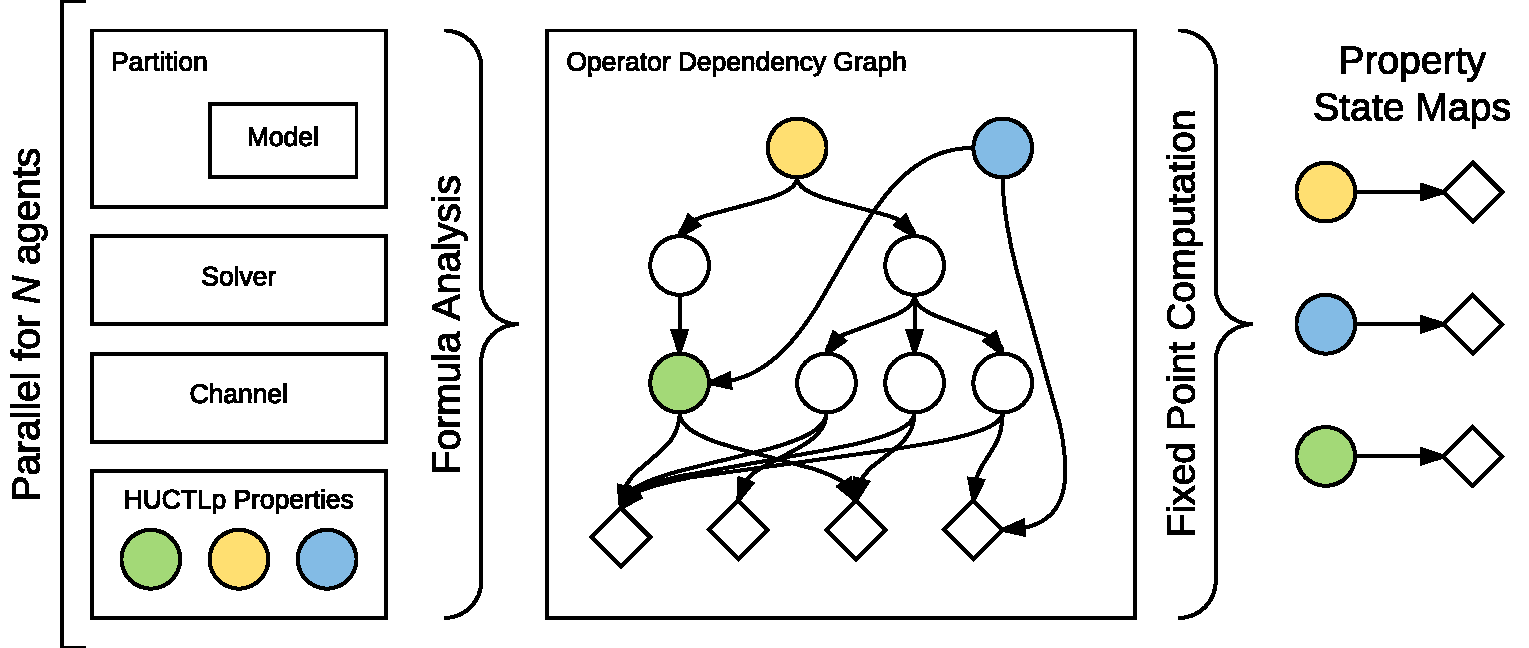
\includegraphics[scale=0.45]{media/core_workflow.pdf}
	\caption{Work flow of the main parameter synthesis module. Circles represent \ac{HUCTLp} operator objects, diamonds \texttt{StateMap}s. }
	\label{fig:core_workflow}
\end{figure}

With all necessary data structures in place, the parameter synthesis engine accepts a set of investigated \ac{HUCTLp} properties and is ready to perform the main procedure. The work flow is depicted in figure \ref{fig:core_workflow}.

The implementation starts by constructing a dependency graph based on the provided \ac{HUCTLp} properties. Each node in the graph is represented by a special operator object which implements the logic of the semantic function $\mathcal{C}$ for one specific \ac{HUCTLp} operator. 

This construction ensures that whenever two properties share a common sub-formula, it is only computed once. Furthermore, this construction also unrolls the state variable valuation, so that for example a property $\hctlAt{x} \varphi$ is represented as $|\dtsS|$ distinct operators, depending on the value of $x$. 


This allows us to ensure that unused valuations don't create unnecessary operators. A good example of such case is a formula $\hctlBind{x} \ctlA\ctlF (\neg x \land \ctlE\ctlF p)$ where $p$ is some atomic proposition. In this case, $\ctlE\ctlF$ is independent on the valuation of $x$, and therefore can be represented by a single operator node in the dependency graph, while the $\ctlA\ctlF$ is unrolled into multiple operators depending on the value of $x$.

Another important optimisation this construction allows is canonisation of the state variable names. This means that if you consider a formula such as $[\hctlBind{x} \ctlA\ctlF x] \lor [\hctlExists{y} (\ctlA \ctlF y \land \neg y)]$, both $\ctlA\ctlF x$ and $\ctlA\ctlF y$ are resolved as the same operator object and are computed only once. 

After the operator dependency graph is constructed, the fixed point algorithm iteratively processes operators in the graph, starting from the smallest (propositions). We always process only one operator at a time, even though this reduces the potential for parallelism. One reason for this is to avoid unnecessary propagation of incomplete results (when a sub-formula of $\ctlE\ctlF$ is updated, this can potentially trigger update in the whole system). Second reason is to reduce the memory requirements. When you only process one operator at a time, you can quickly discard results that are no longer needed, keeping the memory consumption polynomial instead of exponential in the size of the state space (of course, the operator graph can still be exponential, however, we assume that pending operators can be represented very compactly, as opposed to the actual assumption functions).  

As a result of this operation, user obtains a set of \texttt{StateMap}s which represent the parameter synthesis result for the local states of the fragment for each requested property, as depicted in the third part of the work flow figure.

\section{ODE Model Module}


\begin{figure}[]
	\centering
	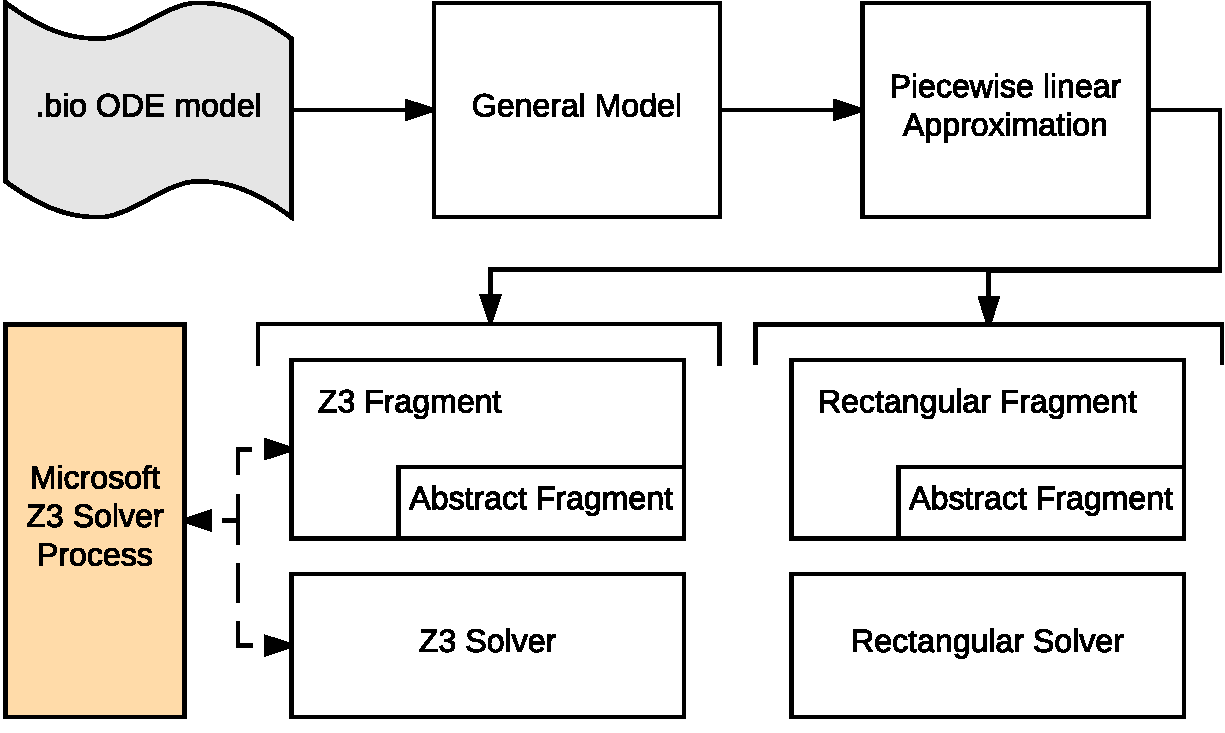
\includegraphics[scale=0.45]{media/ode_workflow.pdf}
	\caption{Work flow of the ode module module. The usage of a specific fragment implementation depends on the properties of the model. }
	\label{fig:ode_workflow}
\end{figure}

The ODE model module provides implementations for working with various types of models based on ordinary differential equations. It relies on the abstraction procedure described in \cite{abs, absOverview} when transforming the continuous equations into a discrete state space. The models are originally represented using a .bio model format (grammar provided in ANTLR4 syntax in the digital appendix) and this module is responsible for parsing the model file, computing the piecewise linear approximation and transforming the model into \ac{PDTS} fragments that can be then used by the main parameter synthesis module. The module also provides appropriate solvers for the supported model types.	

The work flow of this process, with all of it's main components is depicted in figure \ref{fig:ode_workflow}. After the piecewise linear approximation is constructed, the model is analysed for relationships between parameters and an appropriate parameter representation is chosen.

\texttt{Rectangular Model} and the corresponding \texttt{Rectangular Solver} are chosen when the parameters are fully independent (at most one parameter per equation). This type of parameter representation uses a set of hyper-rectangles to encode the parameter constrain and is fairly straightforward and efficient.

\texttt{Z3 Model} and \texttt{Z3 Solver} are then used for more complex models. In this case, the parameter constrains are represented directly as Microsoft Z3 compatible formulae and the SMT solver is directly responsible for deciding satisfiability and formula simplification. This is facilitated by directly interfacing with a Z3 process running in interactive mode. Z3 also provides a direct API for common programming languages. However, we choose not to use this, because it causes problems with parallelism on multi-core machines. 

At the time of writing, Z3 was designed in a way that even for formulae which belong to completely separate contexts, some non-trivial synchronisation is performed. This synchronisation then significantly cripples the parallel execution to a point where adding more concurrent workers actually slows down the execution significantly. Having a set of independent (at the system level) solver processes then enables us to scale the execution on multi-core machines, even though it introduces more overhead and complexity to the whole program.

Finally, this module also provides an \texttt{Abstract Model} class which implements general logic for generating transitions in ODE based models. One can use this class to quickly implement new model variants. All that needs to be provided is a method producing a parameter constrain under which is a given equation at a given vertex positive or negative (corresponding to a positive or negative derivation). Other logic and optimisations (caching, etc.) is then handled solely by the abstract implementation. Naturally, an appropriate solver also has to be provided.

\section{Command line frontend}

\begin{figure}[]
	\centering
	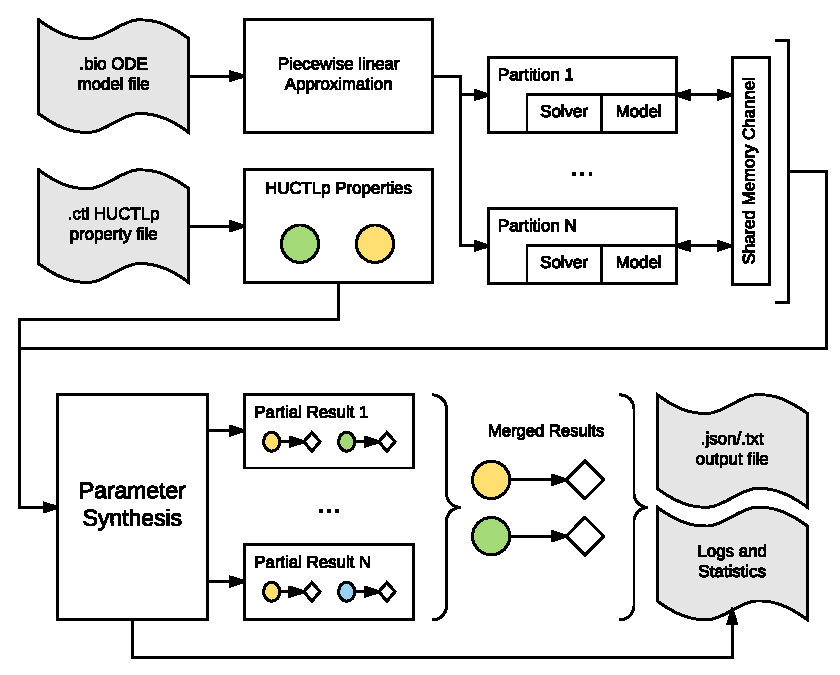
\includegraphics[scale=0.9]{media/cli_workflow.pdf}
	\caption{Work flow of the command line front-end. }
	\label{fig:cli_workflow}
\end{figure}

The command line front-end connects all these modules into one package with a well defined input and output. Schematic description of this module is given in Figure \ref{fig:cli_workflow}.

The process starts by parsing given input files and creating $N$ independent partitions connected using a shared memory communication channel. These data structures are then passed into the parameter synthesis engine.

As soon as the parameter synthesis is finished, the front-end module obtains $N$ partial results from the synthesis engine. These partial results are then merged into one general result set. Finally, the result set can be exported using two supported output formats. First format provides export into a machine readable .json file, suitable for further post-processing or visualisations. Second format provides a more human readable text format, which can be useful when debugging or working with simple models.

The actual content of both formats depends on the type of parameter representation used by the model. When working with hyper-rectangular parameter representation, a parameter constrain is represented using a suitable multi dimensional array interpreted directly as a set of hyper-rectangles. On the other hand, when working with the pure SMT approach, a parameter constrain is represented as a SMT-LIB 2 formula \cite{smtlib}.

Finally, a set of diagnostic and benchmarking data is collected during the computation. These include the amount and frequency of data transfers between partitions (to monitor possible communication bottlenecks) and the average solver throughput (corresponds to the complexity of parameter constrains which were encountered during the computation). These data are generally printed directly to the standard output or can be easily redirected into a separate file.

For a detailed description of the command line arguments accepted by the front-end module, see the tool manual provided as a digital appendix.



\chapter{Evaluation}
\label{chap:evaluation}

In this chapter, we provide evidence to support the claim that our algorithm scales well with increasing amount of computational resources, and that the algorithm is useful, meaning it can provide interesting, non trivial information about the studied model.

\section{Models}

In order to evaluate the algorithm, we first need to define some non-trivial models which we will use to do so. These models, coming from the field of systems biology, are described in this section.

All of the models can be scaled in terms of state and parameter space cardinality by increasing the precision of the piecewise linear approximation.

\subsection{Bi-stable repressilator}

The first model to be considered is the smallest repressilator motif, studied in~\cite{brim2015high,dilao}. It includes two nodes which inhibit each other (see Figure \ref{fig:2Drep} (left)). In biology, this motif is very often present in gene regulatory networks, where $X$ represents product of $gene X$ which inhibits production of $gene Y$ and vice versa.

There are several ways to parametrise this model. In this work, we choose $\phi_X$ and $\phi_Y$ as our parameters, each in the $(0, 1)$ interval (unless explicitly stated otherwise).

\begin{figure}
	\centering
	\begin{center}
		\vspace*{-6mm}
		\hspace*{-1cm}  
		\parbox{4cm}{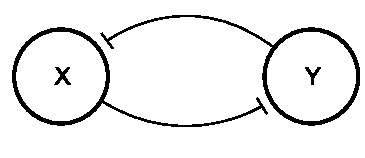
\includegraphics[scale=.6]{2Drep.pdf}}~
		\parbox{6cm}{
			$$\begin{array}{c@{$\,=\,$}l}
			\frac{d[X]}{dt} & k_1 \frac{K_{1}^{n_1}}{K_{1}^{n_1}+[Y]^{n_1}} - \phi_{X}[X]\\[3mm]
			\frac{d[Y]}{dt} & k_2 \frac{K_{2}^{n_2}}{K_{2}^{n_2}+[X]^{n_2}} - \phi_{Y}[Y]
			\end{array}$$
			\center
			$k_1=k_2=1$, $K_{1}=K_{2}=5$, \\
			$n_1=n_2=5$
		}~~
		\vspace*{-5mm}
	\end{center}
	\caption{Bi-stable repressilator regulatory network (left) and its ODE model taken from~\cite{brim2015high} (middle).}
	\vspace*{-0.5em}
	\label{fig:2Drep}
\end{figure}

\subsection{Tri-stable toggle switch}

Tri-stable toggle switch is a model of 3-variable repressilator in which each node inhibits not only one but both of its neighbours (see Figure \ref{fig:3Drep} (left)). Just one of the two ingoing inhibition is enough to repress any entity. Therefore the ODE model possesses multiplication of negative hill function in entity regulation (Fig.~\ref{fig:3Drep} (right)).

Similarly to the bi-stable repressilator, we choose $\phi_X$, $\phi_Y$ and $\phi_Z$ as our parameters, each in the $(0.1, 0.2)$ interval (unless stated otherwise). 

\begin{figure}
	\begin{center}
		% \vspace*{-6mm}
		\hspace*{-1cm}  \parbox{5cm}{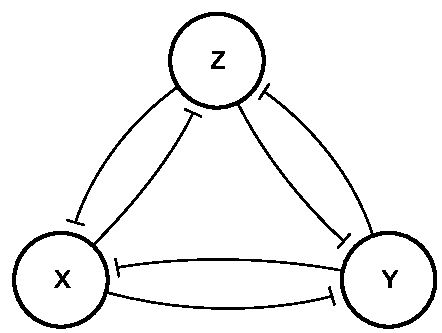
\includegraphics[scale=.6]{triStableRep.pdf}}~
		\parbox{7cm}{
			$$\begin{array}{c@{$\,=\,$}l}
			\frac{d[X]}{dt} & k_{1} \frac{K_{y_1}^{n_1}}{K_{y_1}^{n_1}+[Y]^{n_1}}\cdot \frac{K_{z_1}^{n_2}}{K_{z_1}^{n_2}+[Z]^{n_2}} - \phi_{X}[X]\\[3mm]
			\frac{d[Y]}{dt} & k_{2} \frac{K_{x_2}^{n_3}}{K_{x_2}^{n_3}+[X]^{n_3}} \cdot \frac{K_{z_2}^{n_4}}{K_{z_2}^{n_4}+[Z]^{n_4}} - \phi_{Y}[Y]\\[3mm]
			\frac{d[Z]}{dt} & k_{3} \frac{K_{x_3}^{n_5}}{K_{x_3}^{n_5}+[X]^{n_5}}\cdot \frac{K_{y_3}^{n_6}}{K_{y_3}^{n_6}+[Y]^{n_6}} - \phi_{Z}[Z]
			\end{array}$$
			\center
			$\forall i,j; k_{i}=1$,\\ $K_{x_i}=K_{y_i}=K_{z_i}=5$, 
			$n_j=5$
		}\\
		%\vspace*{-5mm}
	\end{center}
	\caption{Tri-stable toggle switch regulatory network and its ODE model.}
	%\vspace*{-0.5em}
	\label{fig:3Drep}
\end{figure}

\section{Scalability}

\section{Applicability}

To demonstrate the applicability of our approach, we provide an analysis of the stable states of our models, as discovered by the algorithm.

\subsubsection{\textbf{Properties}}

We will study two types of stability motifs. First is a terminal strongly connected component, which can be represented using the \ac{HUCTLp} formula $tSCC = \hctlBind{x} \future\ctlA\ctlG \future\ctlE\ctlF x$. Intuitively, a terminal strongly connected component is a maximal set of states that are pairwise reachable (meaning from any state, I can reach the whole component, but nothing else).

Second motif is a terminal cycle, represented using the formula $tCycle = \hctlBind{x} \future\ctlA\ctlX \future\ctlA\ctlF$. Intuitively, a terminal cycle is a stronger requirement than a terminal component, since the component can contain multiple interleaving cycles, while the terminal cycle property explicitly specifies that there is exactly one cycle (otherwise the $\ctlA$ requirement would be broken).

Notice that we would expect each model to have at least one terminal strongly connected component, however, no such requirement can be imposed to terminal cycles.

In order to show that there are at least two distinct instances of the studied patterns (either $tSCC$ or $tCycle$) in the model, we use the following property: $biPattern = \hctlBind{x} \hctlExists{z \in pattern} pattern \land \neg \future\ctlE\ctlF z$. This property holds in states where the $pattern$ is satisfied and there exists other state (also satisfying $pattern$) not reachable from this state. This is implies presence of two instances, since both our patterns are terminal. Also notice the use of the $exists-in$ operator, which guarantees only appropriate $z$ are considered, thus simplifying the property description and computation performance. Such formula can be further generalised to imply presence of three distinct instances if needed.

Similarly, we can be interested in presence of exactly one instance of the studied pattern. To this end, we can simply use the property $single = pattern \land \neg biPattern$.

\subsubsection{\textbf{Bi-stable repressilator}}

The results of our analysis for the bi-stable repressilator are presented in Figures \ref{fig:biSCC} and \ref{fig:biCycle}. Each figure contains a state space plot and a parameter space plot, where green colour signifies the presence of exactly one pattern instance and the yellow colour signifies presence of exactly two pattern instances. Furthermore, in the state space plot, the mixture of green and yellow represents that either one or two instances of the studied pattern are present, depending on the parameter valuation.

The results of our terminal component analysis are presented in Figure \ref{fig:biSCC}. As expected, the model contains either one or two terminal components, depending on the parameter valuation. Furthermore, the location of these components is clearly visible in the state space plot (right). 

The analysis of the terminal cycles is presented in Figure \ref{fig:biCycle}. As we can see, the model contains parameter valuations for which no terminal cycle is present. For these valuations a manual inspection revealed that multiple non-terminal cycles are present in the model.

\begin{figure}
	
	\begin{center}
		\begin{overpic}[width=.5\textwidth]{results/2D/scc_state.png}\end{overpic}\hfill
		\begin{overpic}[width=.5\textwidth]{results/2D/scc_param.png}\end{overpic}\hfill
	\end{center}
	
	\caption{Presence of two terminal strongly connected components in the bi-stable repressilator model. The parameter space (right) has been zoomed to cover only the interesting area.  }
	\label{fig:biSCC}
\end{figure}

\begin{figure}
	
	\begin{center}
		\begin{overpic}[width=.5\textwidth]{results/2D/cycle_state.png}\end{overpic}\hfill
		\begin{overpic}[width=.5\textwidth]{results/2D/cycle_param.png}\end{overpic}\hfill
	\end{center}
	
	\caption{Presence of two terminal cycles in the bi-stable repressilator model.}
	\label{fig:biCycle}
\end{figure}

\subsubsection{\textbf{Tri-stable toggle switch}}

The results of the analysis for the tri-stable toggle switch are presented in Figures .... The colouring scheme follows similar rules as in the case of the bi-stable repressilator 

\begin{figure}
	
	\begin{center}
		\begin{overpic}[width=.5\textwidth]{results/2D/scc_state.png}\end{overpic}\hfill
		\begin{overpic}[width=.5\textwidth]{results/2D/scc_param.png}\end{overpic}\hfill
	\end{center}
	
	\caption{Presence of two terminal strongly connected components in the bi-stable repressilator model. The parameter space (right) has been zoomed to cover only the interesting area.  }
	\label{fig:triSCC}
\end{figure}

\begin{figure}
	
	\begin{center}
		\begin{overpic}[width=.5\textwidth]{results/2D/cycle_state.png}\end{overpic}\hfill
		\begin{overpic}[width=.5\textwidth]{results/2D/cycle_param.png}\end{overpic}\hfill
	\end{center}
	
	\caption{Presence of two terminal cycles in the bi-stable repressilator model.}
	\label{fig:triCycle}
\end{figure}

\chapter{Conclusion}
\label{chap:conclusions}
In this work, we presented an efficient distributed fixed point algorithm for solving the parameter synthesis problem for \acf{PDTS} with properties specified using the \acf{HUCTLp}. The algorithm works in a semi-symbolic manner, with explicit state space and symbolic parameter space representations, relying on an appropriate solver for deciding and simplifying the parameter sets. 

\ac{HUCTLp} is a more expressive extension of \ac{CTL}, which allows specification of various interesting properties, such as strongly connected components, cycles or directed runs. We provide a detailed discussion of its semantics and its relationship with \ac{CTL}.

We also provide an implementation of the above mentioned algorithm, which is optimised for multi-core usage. The implementation is freely available as part of the Pithya parameter synthesis tool. As a modelling framework, the implementation provides a module for working with ordinary differential equation based models. However, the core algorithm is completely model agnostic. We also provide a bridge to the Microsoft Z3 solver and various domain-specific optimised solvers.

For this implementation, we provide a case study which explores the terminal components and terminal cycles of two well know models from systems biology. We also provide a scalability analysis which shows that the algorithm is able to utilise provided computational resources.

As future work, we would like to extend the implementation with distributed computation capabilities, since the main framework is already prepared for this, only an appropriate \texttt{Communicator} is needed. Other possible research direction would be to design a more general, fixed point computation framework, which can then be used to implement other common algorithms, such as more efficient component detection. One can also consider a cloud oriented approach to the current fixed point algorithm, relying on stream processing. Finally, the implementation would greatly benefit from more domain specific solvers and on-the-fly compilation of models, which would speed up the parameter set related operations and state space generation.

\printbibliography[heading=bibintoc] %% Print the bibliography.

%\bibliographystyle{ieeetr}  
%\bibliography{main}

\appendix
\chapter{List of electronic attachments}
\begin{itemize}
	\item Current source code of the Pithya tool implementing the algorithm.
	\item Pithya manual with description of the input/output formats.
	\item Raw case study results.
\end{itemize}

\end{document}
